\immediate\write18{tex spath3.dtx}
\documentclass{article}
\usepackage{tabularx}
\usepackage{tikz}
\usetikzlibrary{decorations.pathreplacing,calligraphy,matrix}

\makeatletter
\ExplSyntaxOn

\cs_new_nopar:Npn \test_it #1#2
{
  \message{Got~ #1~ and~ #2}
}

\tl_set:Nn \l_tmpa_tl {{20pt}{30pt}}

\exp_last_unbraced:NV \pgfqpoint \l_tmpa_tl

\showthe\pgf@x
\showthe\pgf@y

%\relax\relax\relax

\ExplSyntaxOff
\makeatother

\makeatletter
\def\showpath{%
  \def\pgfqpoint##1##2{(##1, ##2)}%
  \def\pgfsyssoftpath@movetotoken##1##2{%
    \string\pgfsyssoftpath@movetotoken\{##1\}\{##2\}
  }%
  \def\pgfsyssoftpath@linetotoken##1##2{%
    \string\pgfsyssoftpath@linetotoken\{##1\}\{##2\}
  }%
  \def\pgfsyssoftpath@curvetotoken##1##2{%
    \string\pgfsyssoftpath@curvetotoken\{##1\}\{##2\}
  }%
  \def\pgfsyssoftpath@curvetosupportatoken##1##2{%
    \string\pgfsyssoftpath@curvetosupportatoken\{##1\}\{##2\}
  }%
  \def\pgfsyssoftpath@curvetosupportbtoken##1##2{%
    \string\pgfsyssoftpath@curvetosupportbtoken\{##1\}\{##2\}
  }%
}

\tikzset{save as spath/.code={%
  \tikz@addmode{\pgfsyssoftpath@getcurrentpath\spath@tmp@path\MakeSPath{#1}{\spath@tmp@path}}}}

\tikzset{save as spath list/.code={%
    \tikz@addmode{\pgfsyssoftpath@getcurrentpath\spath@tmp@path\MakeSPathList{#1}{\spath@tmp@path}}}}


\tikzset{
  restore spath/.code={%
    \SPathInfoInto{#1}{minbb}{\spath@tmp@pt}%
    \expandafter\pgfqpoint\spath@tmp@pt
    \pgf@protocolsizes\pgf@x\pgf@y
    \SPathInfoInto{#1}{maxbb}{\spath@tmp@pt}%
    \expandafter\pgfqpoint\spath@tmp@pt
    \pgf@protocolsizes\pgf@x\pgf@y
    \SPathInfoInto{#1}{path}{\spath@tmp@path}%
    \pgfsyssoftpath@setcurrentpath\spath@tmp@path
  }
}
\makeatother

\newcommand\displaypath[1]{%

Displaying path information for: #1

\begin{tabularx}{\textwidth}{r@{:\hskip\arraycolsep}X}
Length & \SPathInfo{#1}{length} \\
Real length & \SPathInfo{#1}{reallength} \\
Number of components & \SPathInfo{#1}{numberofcomponents} \\
Initial point & \showpath\SPathInfoInto{#1}{initialpoint}{\stuff}\expandafter\pgfqpoint\stuff \\
Final point & \showpath\SPathInfoInto{#1}{finalpoint}{\stuff}\expandafter\pgfqpoint\stuff \\
Final action & \texttt{\showpath\SPathInfo{#1}{finalaction}} \\
Path & \texttt{\showpath\SPathInfo{#1}{path}} \\
Reverse path & \texttt{\showpath\SPathInfo{#1}{reversepath}} \\
Final point & \showpath\SPathInfoInto{#1}{finalpoint}{\stuff}\expandafter\pgfqpoint\stuff \\
Initial action & \texttt{\showpath\SPathInfo{#1}{initialaction}} \\
Final action & \texttt{\showpath\SPathInfo{#1}{finalaction}} \\
Min bb & \showpath\SPathInfoInto{#1}{minbb}{\stuff}\expandafter\pgfqpoint\stuff \\
Max bb & \showpath\SPathInfoInto{#1}{maxbb}{\stuff}\expandafter\pgfqpoint\stuff \\
\end{tabularx}%
}

\begin{document}

\tikz \calligraphy[copperplate] (0,0) .. controls +(1,-1) and +(-1,1) .. ++(3,0) [this stroke style={light,taper=start}] +(0,0) .. controls +(1,-1) and +(-1,1) .. ++(3,0) [this stroke style={taper,heavy}];

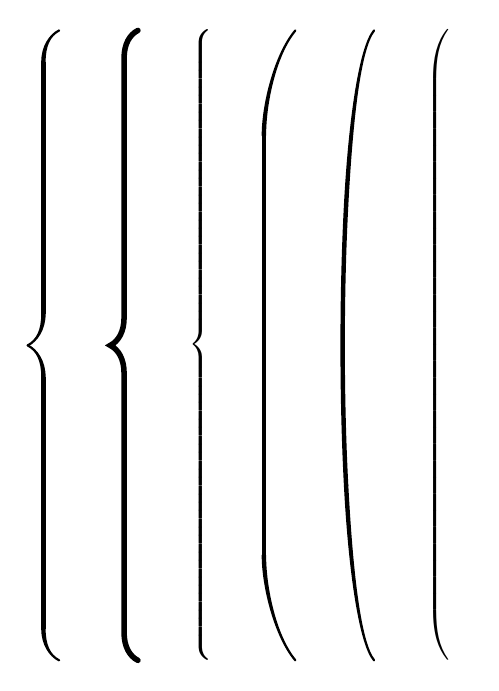
\begin{tikzpicture}
\draw[decorate,decoration={calligraphic brace,amplitude=4mm},ultra thick] (0,0) -- (0,8);
\draw[line width=2pt,decorate,decoration={brace,amplitude=10},line cap=round] (1,0) -- ++(0,8);
\node[anchor=south west,minimum height=8cm,outer sep=0pt,left delimiter=\{] (a) at (2,0) {};
\draw[decorate,decoration={calligraphic straight parenthesis,amplitude=4mm},ultra thick] (3,0) -- ++(0,8);
\draw[decorate,decoration={calligraphic curved parenthesis,amplitude=4mm},ultra thick] (4,0) -- ++(0,8);
\node[anchor=south west,minimum height=8cm,outer sep=0pt,left delimiter=(] (a) at (5,0) {};
\end{tikzpicture}



\begin{tikzpicture}
\draw[save as spath=my path] (0,0) -- (1,1) .. controls +(1,0) and +(-1,0) .. (3,0);
\end{tikzpicture}

\bigskip

\SPathPrepare{my path}

\displaypath{my path}

\SPathTranslateInto {my path} {translated path} {10pt} {-10pt}

\displaypath{translated path}

\SPathWeldInto {my path} {weld path} {translated path}

\displaypath{weld path}

\begin{tikzpicture}
\draw[restore spath=my path];
\end{tikzpicture}

\begin{tikzpicture}
\draw[restore spath=weld path];
\end{tikzpicture}

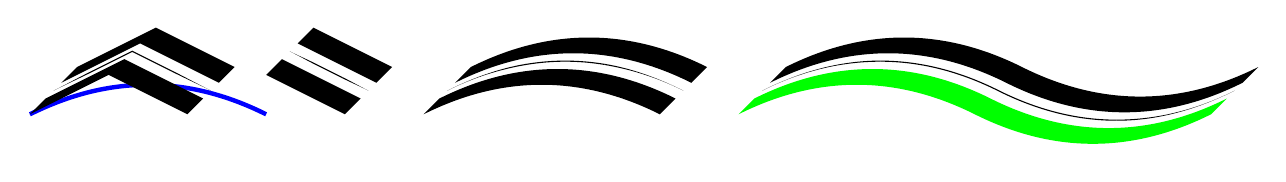
\begin{tikzpicture}
\draw[define pen,red,ultra thick] (0,0) -- (.2,.2) (.3,.3) (.4,.4) -- (.6,.6);
\draw[blue,ultra thick] (0,0) .. controls +(1,.5) and +(-1,.5) .. (3,0);
%\draw[shift={(1cm,1cm)},use pen,pen colour=green] (0,0) .. controls +(1,.5) and +(-1,.5) .. (3,0) (4,0) -- (4,1);
\draw[use pen] (0,0) -- (1,.5) -- (2,0);
\draw[use pen] (3,.5) -- (4,0);
\draw[use pen] (5,0) .. controls +(1,.5) and +(-1,.5) .. +(3,0);
\draw[use pen,nib style={1}{pen colour=green}] (9,0) .. controls +(1,.5) and +(-1,.5) .. ++(3,0) .. controls +(1,-.5) and +(-1,-.5) .. ++(3,0);
\end{tikzpicture}

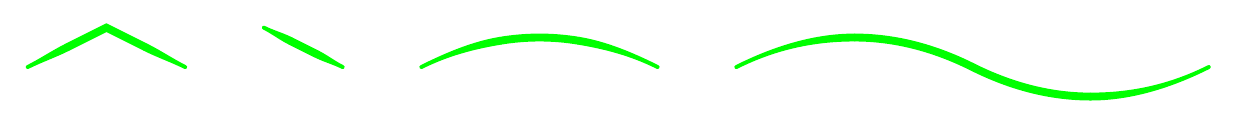
\begin{tikzpicture}
\begin{scope}[every path/.append style={use pen=copperplate,line width=1mm,pen colour=green,taper,taper width=.5mm}]
\draw (0,0) -- (1,.5) -- (2,0);
\draw (3,.5) -- (4,0);
\draw (5,0) .. controls +(1,.5) and +(-1,.5) .. +(3,0);
\draw (9,0) .. controls +(1,.5) and +(-1,.5) .. ++(3,0) .. controls +(1,-.5) and +(-1,-.5) .. ++(3,0);
\end{scope}
\end{tikzpicture}

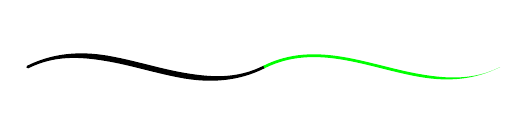
\begin{tikzpicture}
\draw[use pen=copperplate,taper,stroke style={1}{heavy},light,stroke style={2}{taper start=false}] (0,0) .. controls +(1,.5) and +(-1,-.5) .. ++(3,0) ++(0,0) [this stroke style={pen colour=green}] .. controls +(1,.5) and +(-1,-.5) .. ++(3,0);
\end{tikzpicture}


\end{document}